% =====================================================================
%  Analysis of Algorithms – Lab 06
%  Full Report: Recurrences, Merge Sort & Quick Sort
% =====================================================================
\documentclass[12pt,a4paper]{article}

% ----- Encoding & Language -------------------------------------------
\usepackage[utf8]{inputenc}
\usepackage[T1]{fontenc}
\usepackage[english]{babel}

% ----- Page layout ---------------------------------------------------
\usepackage{geometry}
\geometry{top=2.5cm,bottom=2.5cm,left=2.8cm,right=2.8cm}

% ----- Math ----------------------------------------------------------
\usepackage{amsmath,amssymb,amsthm}
\usepackage{mathtools}

% ----- Code listings -------------------------------------------------
\usepackage{listings}
\usepackage[dvipsnames]{xcolor}

% ----- Graphics & floats ---------------------------------------------
\usepackage{graphicx}
\usepackage{float}
\usepackage{tikz}
\usetikzlibrary{arrows.meta, positioning, shapes.geometric, calc}

% ----- Tables --------------------------------------------------------
\usepackage{booktabs}
\usepackage{array}
\usepackage{multirow}

% ----- Layout helpers ------------------------------------------------
\usepackage{enumitem}
\usepackage{fancyhdr}
\setlength{\headheight}{25pt}
\usepackage{titlesec}
\usepackage{parskip}
\usepackage{mdframed}
\usepackage{caption}
\usepackage{subcaption}
\usepackage{setspace}
\usepackage{hyperref}
\hypersetup{colorlinks=true,linkcolor=NavyBlue,urlcolor=NavyBlue,citecolor=NavyBlue}
% (removed duplicate xcolor)

% =====================================================================
%  Colour palette
% =====================================================================
\definecolor{primary}{RGB}{20,60,120}       % deep navy
\definecolor{accent}{RGB}{0,120,180}        % teal-blue
\definecolor{lightbg}{RGB}{247,249,252}     % near-white
\definecolor{codebg}{RGB}{245,245,245}
\definecolor{codegreen}{RGB}{30,130,30}
\definecolor{codegray}{RGB}{120,120,120}
\definecolor{codepurple}{RGB}{130,0,160}
\definecolor{codeblue}{RGB}{0,0,200}
\definecolor{outputbg}{RGB}{240,248,240}
\definecolor{outputborder}{RGB}{100,160,100}
\definecolor{warningbg}{RGB}{255,250,230}
\definecolor{warningborder}{RGB}{200,160,40}

% =====================================================================
%  Listings style
% =====================================================================
\lstdefinestyle{cstyle}{
  backgroundcolor=\color{codebg},
  commentstyle=\color{codegreen}\itshape\small,
  keywordstyle=\color{codeblue}\bfseries,
  numberstyle=\tiny\color{codegray},
  stringstyle=\color{codepurple},
  basicstyle=\ttfamily\footnotesize,
  breakatwhitespace=false,
  breaklines=true,
  captionpos=b,
  keepspaces=true,
  numbers=left,
  numbersep=10pt,
  showstringspaces=false,
  tabsize=4,
  frame=single,
  rulecolor=\color{gray!30},
  xleftmargin=2em,
  framexleftmargin=1.5em,
  aboveskip=8pt,
  belowskip=8pt,
}
\lstset{style=cstyle}

% =====================================================================
%  Theorem environments
% =====================================================================
\theoremstyle{plain}
\newtheorem{theorem}{Theorem}[section]
\newtheorem{lemma}[theorem]{Lemma}
\newtheorem{corollary}[theorem]{Corollary}

\theoremstyle{definition}
\newtheorem{definition}{Definition}[section]

\theoremstyle{remark}
\newtheorem*{remark}{Remark}
\newtheorem*{note}{Note}

% =====================================================================
%  Framed environments for output and key observations
% =====================================================================
\newmdenv[
  backgroundcolor=outputbg,
  linecolor=outputborder,
  linewidth=1.5pt,
  leftmargin=0pt, rightmargin=0pt,
  innerleftmargin=10pt, innerrightmargin=10pt,
  innertopmargin=6pt, innerbottommargin=6pt,
  skipabove=8pt, skipbelow=8pt,
]{outputbox}

\newmdenv[
  backgroundcolor=warningbg,
  linecolor=warningborder,
  linewidth=1.5pt,
  leftmargin=0pt, rightmargin=0pt,
  innerleftmargin=10pt, innerrightmargin=10pt,
  innertopmargin=6pt, innerbottommargin=6pt,
  skipabove=8pt, skipbelow=8pt,
]{keybox}

\newmdenv[
  backgroundcolor=lightbg,
  linecolor=primary!40,
  linewidth=1pt,
  leftmargin=0pt, rightmargin=0pt,
  innerleftmargin=10pt, innerrightmargin=10pt,
  innertopmargin=6pt, innerbottommargin=6pt,
  skipabove=6pt, skipbelow=6pt,
]{infobox}

% =====================================================================
%  Header / footer
% =====================================================================
\pagestyle{fancy}
\fancyhf{}
\fancyhead[L]{\small\color{primary}\textbf{Analysis of Algorithms} \textbar\ Lab 06}
\fancyhead[R]{\small\color{primary}Yachay Tech University}
\fancyfoot[C]{\small\thepage}
\renewcommand{\headrulewidth}{0.5pt}
\renewcommand{\headrule}{\hbox to\headwidth{\color{primary!50}\leaders\hrule height \headrulewidth\hfill}}

% =====================================================================
%  Section formatting
% =====================================================================
\titleformat{\section}
  {\Large\bfseries\color{primary}}
  {\color{accent}Exercise \thesection.}{0.6em}{}
  [{\vspace{2pt}\color{primary!40}\titlerule[0.8pt]\vspace{4pt}}]

\titleformat{\subsection}
  {\bfseries\color{primary!80}}{\thesubsection}{0.5em}{}

\titleformat{\subsubsection}
  {\bfseries\color{primary!60}\itshape}{\thesubsubsection}{0.5em}{}

% =====================================================================
%  Convenience commands
% =====================================================================
\newcommand{\bigO}[1]{\ensuremath{\mathcal{O}(#1)}}
\newcommand{\DAG}{\textsc{dag}}

\begin{document}

% ---------------------------------------------------------------------
%  Institutional Header with Logos
% ---------------------------------------------------------------------
\noindent
\begin{minipage}[c]{0.26\textwidth}
  
\includegraphics[width=\linewidth,height=1.45cm,keepaspectratio]{figures/logo1.png}
\end{minipage}%
\hfill
\begin{minipage}[c]{0.45\textwidth}
  \centering
  {\bfseries\large\color{primary} YACHAY TECH UNIVERSITY}\\[2pt]
  {\footnotesize\bfseries School of Mathematical and Computational Sciences}\\[2pt]
  {\footnotesize\color{primary!80}\textbf{Course:} Analysis of Algorithms \textbar\ Lab 06}
\end{minipage}%
\hfill
\begin{minipage}[c]{0.26\textwidth}
  \raggedleft
  
\includegraphics[width=\linewidth,height=1.45cm,keepaspectratio]{figures/logo2.png}
\end{minipage}

\vspace{0.4em}
{\color{primary}\hrule height 1.2pt}
\vspace{0.8em}

\begin{center}
  {\Large\bfseries\color{primary} Assignment 06: Recurrences, Merge Sort Stability \& Quick Sort}\\[0.4em]
  {\normalsize\textbf{Author:} Darío Pomasqui \quad\textbar\quad \textbf{Date:} \today}\\[3pt]
  {\footnotesize\textbf{GitHub Repository:} \href{https://github.com/your-username/algorithms-lab06}{\texttt{https://github.com/your-username/algorithms-lab06}}}
\end{center}

\vspace{0.8em}

\section{Recurrence Relations via the Master Theorem}

The Master Theorem provides a cookbook method for solving divide-and-conquer recurrences of the canonical form:
\begin{equation}
T(n) = a T\left(\frac{n}{b}\right) + f(n), \quad \text{with } a \ge 1, \; b > 1, \; T(1) = 1
\end{equation}
The asymptotic behavior is governed by comparing the driving function $f(n)$ to the watershed function $n^{\log_b a}$:
\begin{enumerate}
    \item \textbf{Case 1 (Leaf-dominated):} If $f(n) = O\left(n^{\log_b a - \epsilon}\right)$ for some $\epsilon > 0$, then $T(n) = \Theta\left(n^{\log_b a}\right)$.
    \item \textbf{Case 2 (Balanced work):} If $f(n) = \Theta\left(n^{\log_b a} \log^k n\right)$ with $k \ge 0$, then $T(n) = \Theta\left(n^{\log_b a} \log^{k+1} n\right)$.
    \item \textbf{Case 3 (Root-dominated):} If $f(n) = \Omega\left(n^{\log_b a + \epsilon}\right)$ for some $\epsilon > 0$, and if the regularity condition holds: $a f\left(\frac{n}{b}\right) \le c f(n)$ for some constant $c < 1$ and all sufficiently large $n$, then $T(n) = \Theta(f(n))$.
\end{enumerate}

For all three recurrences below, the recurrence parameters are $a = 4$ and $b = 2$, yielding the critical exponent:
\begin{equation}
\log_b a = \log_2 4 = 2 \implies n^{\log_b a} = n^2
\end{equation}

% -----------------------------------------------------------------------------
\subsection{Recurrence 1.1: \texorpdfstring{$T(n) = 4 T(n/2) + n, \quad T(1) = 1$}{T(n) = 4T(n/2) + n, T(1) = 1}}

\paragraph{Master Theorem Formulation:}
Here, $f(n) = n$. We compare $f(n)$ to $n^{\log_b a} = n^2$:
\begin{equation}
f(n) = n = O\left(n^{2 - \epsilon}\right) \quad \text{for } \epsilon = 1 > 0
\end{equation}
Because the work at the leaves dominates the dividing and combining work at the internal nodes, \textbf{Case 1} of the Master Theorem applies directly:
\begin{equation}
\boxed{T(n) = \Theta\left(n^2\right)}
\end{equation}

\paragraph{Verification via Recursion Tree Method:}
At depth $i$ of the recursion tree (where $i = 0$ is the root):
\begin{itemize}
    \item Number of subproblems: $4^i$.
    \item Size of each subproblem: $n / 2^i$.
    \item Work done at level $i$: $4^i \cdot f\left(\frac{n}{2^i}\right) = 4^i \cdot \frac{n}{2^i} = n \cdot 2^i$.
\end{itemize}
Summing over all levels from $i = 0$ to $h = \log_2 n$:
\begin{equation}
T(n) = \sum_{i=0}^{\log_2 n} n \cdot 2^i = n \sum_{i=0}^{\log_2 n} 2^i = n \left(2^{\log_2 n + 1} - 1\right) = n (2n - 1) = 2n^2 - n
\end{equation}
For $n = 1$, $T(1) = 2(1)^2 - 1 = 1$, satisfying the base condition. Asymptotically, $2n^2 - n = \Theta(n^2)$, corroborating the Master Theorem result.

% -----------------------------------------------------------------------------
\subsection{Recurrence 1.2: \texorpdfstring{$T(n) = 4 T(n/2) + n^2, \quad T(1) = 1$}{T(n) = 4T(n/2) + n\textasciicircum 2, T(1) = 1}}

\paragraph{Master Theorem Formulation:}
Here, $f(n) = n^2$. Comparing $f(n)$ to $n^{\log_b a} = n^2$:
\begin{equation}
f(n) = n^2 = \Theta\left(n^{\log_b a} \log^0 n\right)
\end{equation}
Because the work done at each level of the recursion tree is asymptotically equal, \textbf{Case 2} (with $k = 0$) applies:
\begin{equation}
\boxed{T(n) = \Theta\left(n^2 \log n\right)}
\end{equation}

\paragraph{Verification via Recursion Tree Method:}
At level $i$, the total work is:
\begin{equation}
\text{Work}_i = 4^i \cdot \left(\frac{n}{2^i}\right)^2 = 4^i \cdot \frac{n^2}{4^i} = n^2
\end{equation}
Since every single level performs exactly $n^2$ work, and there are $\log_2 n + 1$ levels from root to leaves:
\begin{equation}
T(n) = \sum_{i=0}^{\log_2 n} n^2 = n^2 (\log_2 n + 1) = n^2 \log_2 n + n^2 = \Theta\left(n^2 \log n\right)
\end{equation}
Checking the base case: for $n = 1$, $T(1) = 1^2 (0 + 1) = 1$, matching the base condition.

% -----------------------------------------------------------------------------
\subsection{Recurrence 1.3: \texorpdfstring{$T(n) = 4 T(n/2) + n^3, \quad T(1) = 1$}{T(n) = 4T(n/2) + n\textasciicircum 3, T(1) = 1}}

\paragraph{Master Theorem Formulation:}
Here, $f(n) = n^3$. Comparing $f(n)$ to $n^{\log_b a} = n^2$:
\begin{equation}
f(n) = n^3 = \Omega\left(n^{2 + \epsilon}\right) \quad \text{for } \epsilon = 1 > 0
\end{equation}
To apply \textbf{Case 3}, we must formally verify the regularity condition:
\begin{equation}
a f\left(\frac{n}{b}\right) \le c f(n) \iff 4 \left(\frac{n}{2}\right)^3 \le c n^3 \iff 4 \cdot \frac{n^3}{8} \le c n^3 \iff \frac{1}{2} n^3 \le c n^3
\end{equation}
Choosing $c = \frac{1}{2} < 1$, the condition strictly holds for all $n \ge 1$. Therefore, Case 3 applies:
\begin{equation}
\boxed{T(n) = \Theta\left(n^3\right)}
\end{equation}

\paragraph{Verification via Recursion Tree Method:}
At level $i$, the work is:
\begin{equation}
\text{Work}_i = 4^i \cdot \left(\frac{n}{2^i}\right)^3 = 4^i \cdot \frac{n^3}{8^i} = n^3 \cdot \left(\frac{4}{8}\right)^i = n^3 \cdot \left(\frac{1}{2}\right)^i
\end{equation}
Summing over all levels yields a decaying geometric series:
\begin{equation}
T(n) = n^3 \sum_{i=0}^{\log_2 n} \left(\frac{1}{2}\right)^i = n^3 \left(\frac{1 - (1/2)^{\log_2 n + 1}}{1 - 1/2}\right) = 2 n^3 \left(1 - \frac{1}{2n}\right) = 2 n^3 - n^2
\end{equation}
For $n = 1$, $T(1) = 2(1) - 1 = 1$. Asymptotically, $2 n^3 - n^2 = \Theta(n^3)$.

\begin{table}[h!]
\centering
\small
\setlength{\tabcolsep}{4.5pt}
\caption{Summary of Recurrences Solved via the Master Theorem}
\begin{tabular}{cccccc}
\toprule
\textbf{Recurrence} & $a$ & $b$ & $f(n)$ & \textbf{Master Theorem Case} & \textbf{Solution} $T(n)$ \\
\midrule
$T(n) = 4T(n/2) + n$   & 4 & 2 & $n$   & Case 1 ($f(n) = O(n^{2-1})$) & $\Theta(n^2)$ \\
$T(n) = 4T(n/2) + n^2$ & 4 & 2 & $n^2$ & Case 2 ($f(n) = \Theta(n^2)$) & $\Theta(n^2 \log n)$ \\
$T(n) = 4T(n/2) + n^3$ & 4 & 2 & $n^3$ & Case 3 ($f(n) = \Omega(n^{2+1}), c=\frac{1}{2}$) & $\Theta(n^3)$ \\
\bottomrule
\end{tabular}
\end{table}

\subsection{Handwritten Mathematical Derivations}
To corroborate the analytical steps presented above, Figures~\ref{fig:mano1} and \ref{fig:mano2} display the handwritten resolution of the three recurrences, detailing the step-by-step substitution, critical exponent computation, case categorization according to the Master Theorem, and recursive tree expansions.

\begin{figure}[H]
    \centering
    \begin{subfigure}[b]{0.48\textwidth}
        \centering
        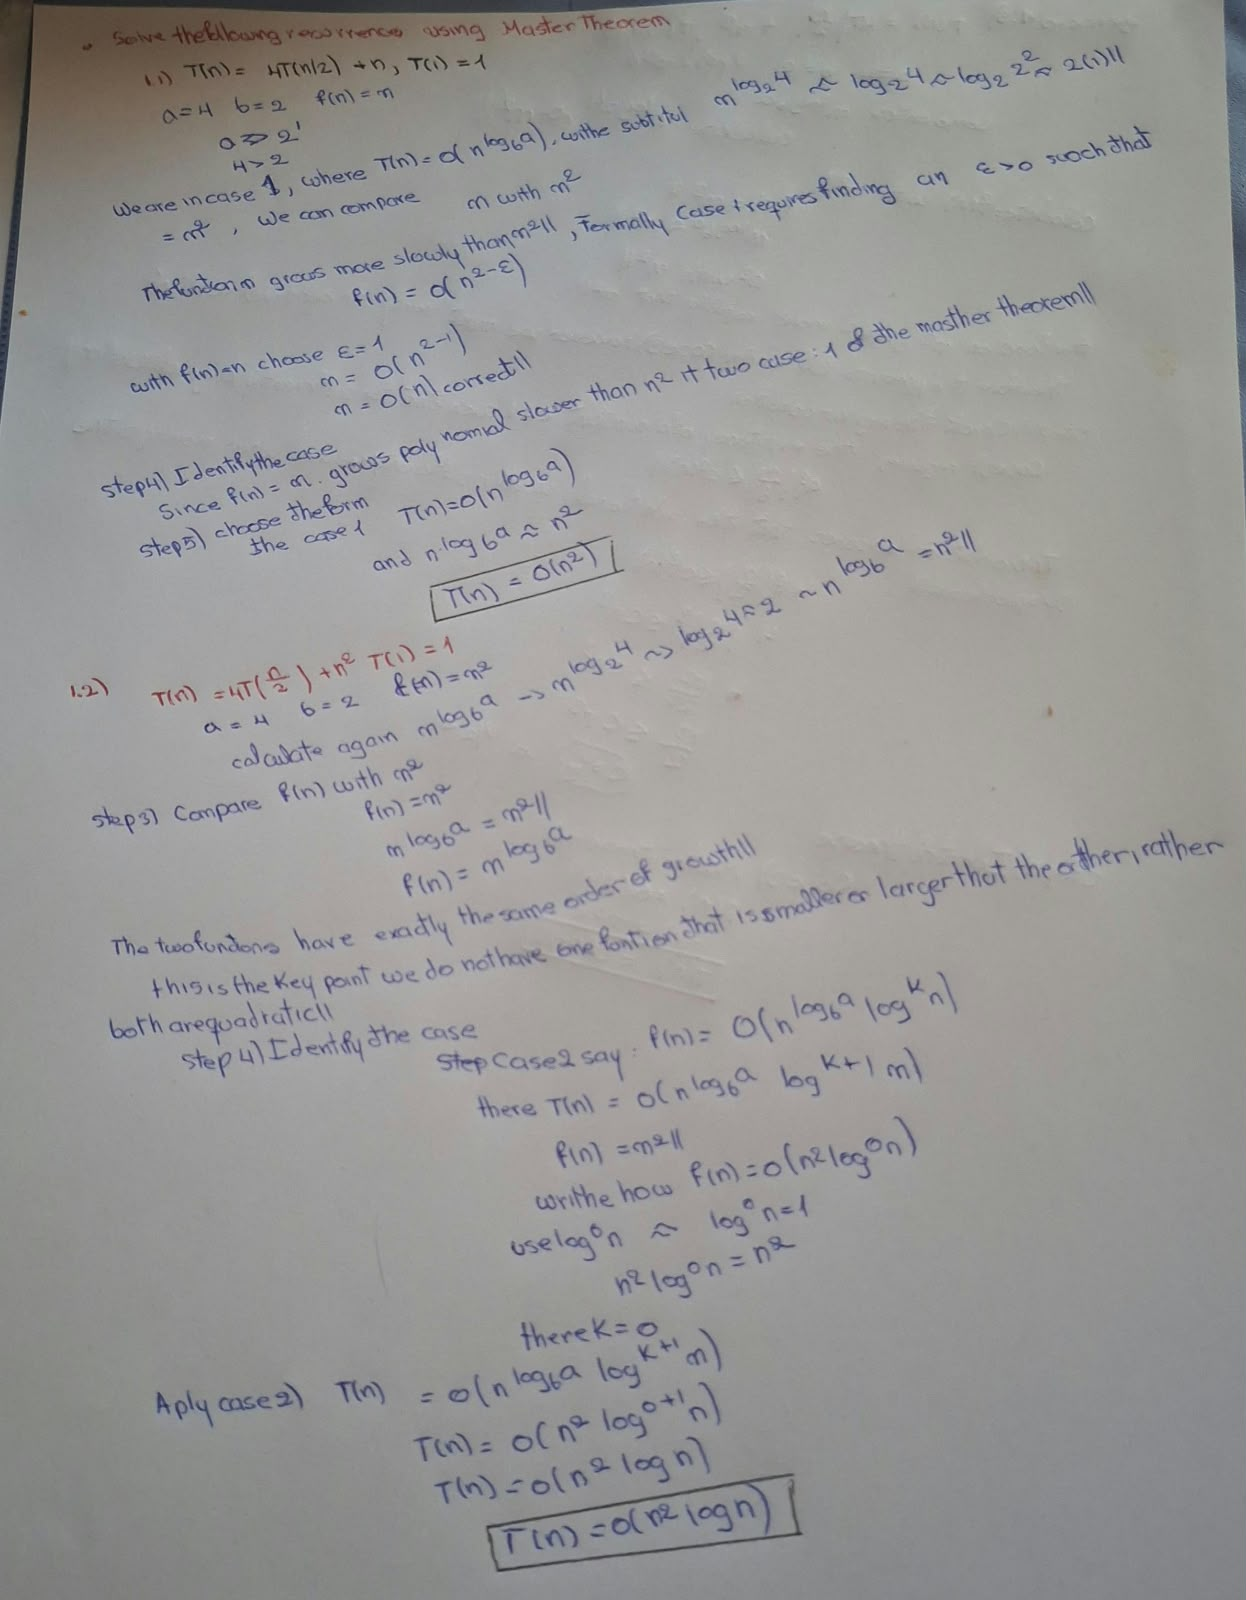
\includegraphics[width=\linewidth,height=8.5cm,keepaspectratio]{figures/parte1-amano.jpeg}
        \caption{Handwritten derivations: Recurrences 1.1 and 1.2.}
        \label{fig:mano1}
    \end{subfigure}
    \hfill
    \begin{subfigure}[b]{0.48\textwidth}
        \centering
        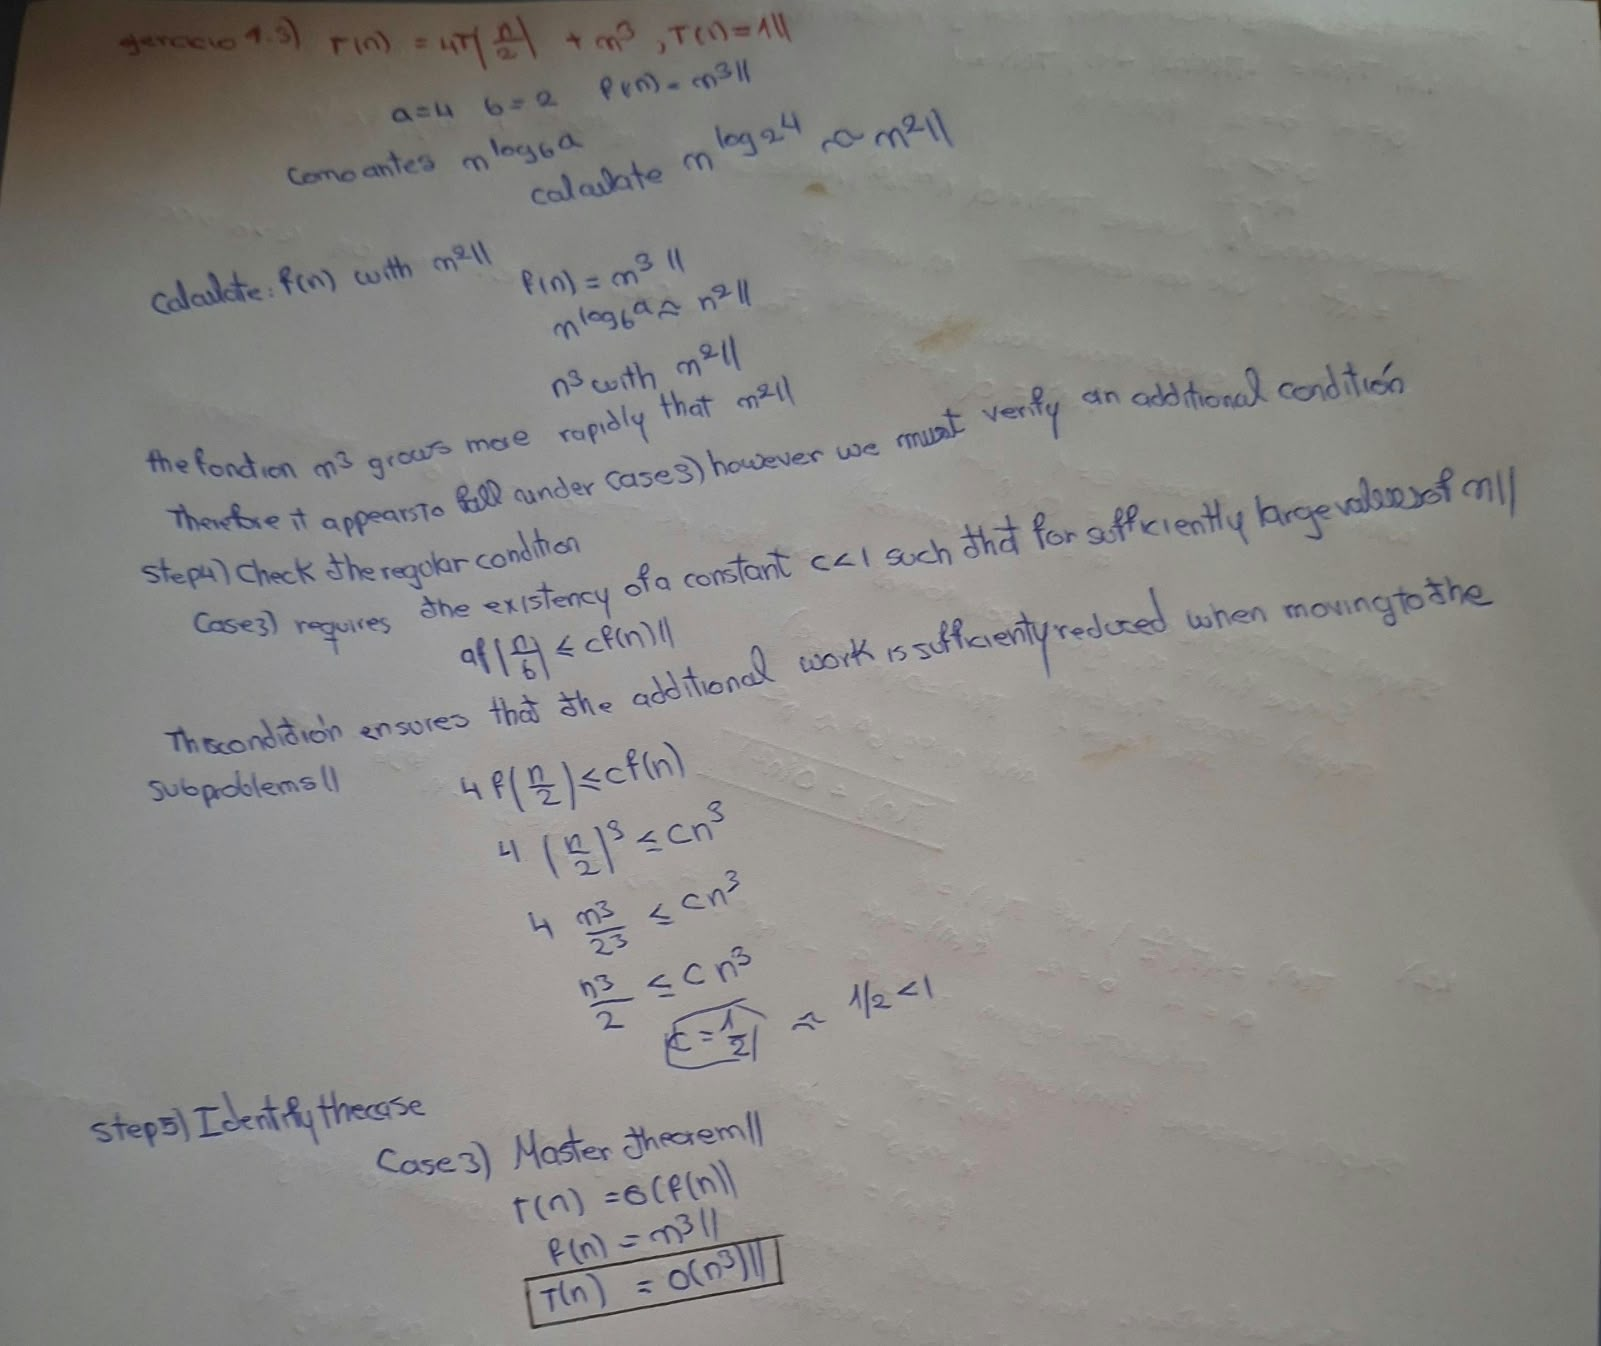
\includegraphics[width=\linewidth,height=8.5cm,keepaspectratio]{figures/parte21-amano.jpeg}
        \caption{Handwritten derivations: Recurrence 1.3 and tree method.}
        \label{fig:mano2}
    \end{subfigure}
    \caption{Photographic evidence of handwritten mathematical solutions for Exercise 1.}
    \label{fig:handwritten_derivations}
\end{figure}

\clearpage
% =============================================================================
\section{Implementation of Merge Sort}

Merge Sort is a quintessential divide-and-conquer algorithm. The input array is divided into two balanced halves until base subarrays of size 1 are reached. Then, during the combine phase, the two sorted subarrays are merged into a single sorted array in linear time.

\begin{lstlisting}[language=C, caption={Merge Sort implementation in C (\texttt{merge\_sort.c})}]
void merge_int(int arr[], int left, int mid, int right) {
    int n1 = mid - left + 1;
    int n2 = right - mid;

    int *L = (int *)malloc(n1 * sizeof(int));
    int *R = (int *)malloc(n2 * sizeof(int));

    for (int i = 0; i < n1; i++) L[i] = arr[left + i];
    for (int j = 0; j < n2; j++) R[j] = arr[mid + 1 + j];

    int i = 0, j = 0, k = left;
    while (i < n1 && j < n2) {
        if (L[i] <= R[j]) {   /* <= preserves stability */
            arr[k++] = L[i++];
        } else {
            arr[k++] = R[j++];
        }
    }
    while (i < n1) arr[k++] = L[i++];
    while (j < n2) arr[k++] = R[j++];

    free(L);
    free(R);
}

void merge_sort_int(int arr[], int left, int right) {
    if (left < right) {
        int mid = left + (right - left) / 2;
        merge_sort_int(arr, left, mid);
        merge_sort_int(arr, mid + 1, right);
        merge_int(arr, left, mid, right);
    }
}
\end{lstlisting}

\paragraph{Complexity Characteristics:}
\begin{itemize}
    \item \textbf{Time Complexity:} Regardless of initial order, the recurrence is $T(n) = 2 T(n/2) + \Theta(n)$. By Master Theorem Case 2, $T(n) = \Theta(n \log n)$ in the worst, best, and average cases.
    \item \textbf{Space Complexity:} Requires $\Theta(n)$ auxiliary memory for temporary buffers during merge.
\end{itemize}

% =============================================================================
\section{Stability Analysis and Experimentation on Merge Sort}

\paragraph{Definition of Stability:}
A sorting algorithm is defined as \textbf{stable} if and only if two elements with equal sorting keys appear in the sorted output in the identical relative order as they occupied in the input array:
\begin{equation}
\forall i < j, \quad \text{if } \text{Key}(A[i]) = \text{Key}(A[j]), \quad \text{then } \text{Pos}_{\text{out}}(A[i]) < \text{Pos}_{\text{out}}(A[j])
\end{equation}

\paragraph{Theoretical Assessment:}
Merge Sort is \textbf{stable} when implemented standardly. The stability is established during the merge routine:
\begin{itemize}
    \item When elements from subarray $L$ and subarray $R$ are compared:
    \begin{equation}
    \text{if } (L[i].\text{key} \le R[j].\text{key}) \implies \text{choose } L[i]
    \end{equation}
    Because elements in $L$ originally appeared before elements in $R$, choosing $L[i]$ on ties guarantees that equal elements originating earlier in the sequence are placed first.
    \item If the programmer erroneously writes $L[i].\text{key} < R[j].\text{key}$, then upon equality, the element from $R$ is selected first, reversing their original order and rendering the sort \textit{unstable}.
\end{itemize}

\paragraph{Empirical Demonstration:}
To experimentally verify stability, we define a structure consisting of a sorting \texttt{key}, an instance \texttt{tag}, and the record's \texttt{original\_pos}:
\begin{lstlisting}[language=C]
typedef struct {
    int key;
    char tag;
    int original_pos;
} Element;
\end{lstlisting}

We construct an input array containing multiple identical keys:
\begin{equation}
\text{Input} = [(5, \text{'A'}, 0), \; (3, \text{'A'}, 1), \; (5, \text{'B'}, 2), \; (2, \text{'A'}, 3), \; (5, \text{'C'}, 4), \; (1, \text{'A'}, 5), \; (3, \text{'B'}, 6)]
\end{equation}

\paragraph{Observed Experimental Results:}
\begin{enumerate}
    \item \textbf{Standard Merge Sort (with $\le$):}
    \begin{equation}
    \text{Output} = [(1, \text{'A'}), (2, \text{'A'}), \mathbf{(3, \text{'A'}, 1), (3, \text{'B'}, 6)}, \mathbf{(5, \text{'A'}, 0), (5, \text{'B'}, 2), (5, \text{'C'}, 4)}]
    \end{equation}
    The relative sequence $5\text{A} \to 5\text{B} \to 5\text{C}$ (original indices $0 < 2 < 4$) and $3\text{A} \to 3\text{B}$ ($1 < 6$) are preserved. The sort is confirmed \textbf{STABLE}.
    
    \item \textbf{Control Test (with $<$ condition):}
    \begin{equation}
    \text{Output} = [(1, \text{'A'}), (2, \text{'A'}), \mathbf{(3, \text{'B'}, 6), (3, \text{'A'}, 1)}, \mathbf{(5, \text{'C'}, 4), (5, \text{'B'}, 2), (5, \text{'A'}, 0)}]
    \end{equation}
    The identical keys have been inverted, confirming that tie handling governs algorithmic stability.
\end{enumerate}

\begin{figure}[H]
\centering
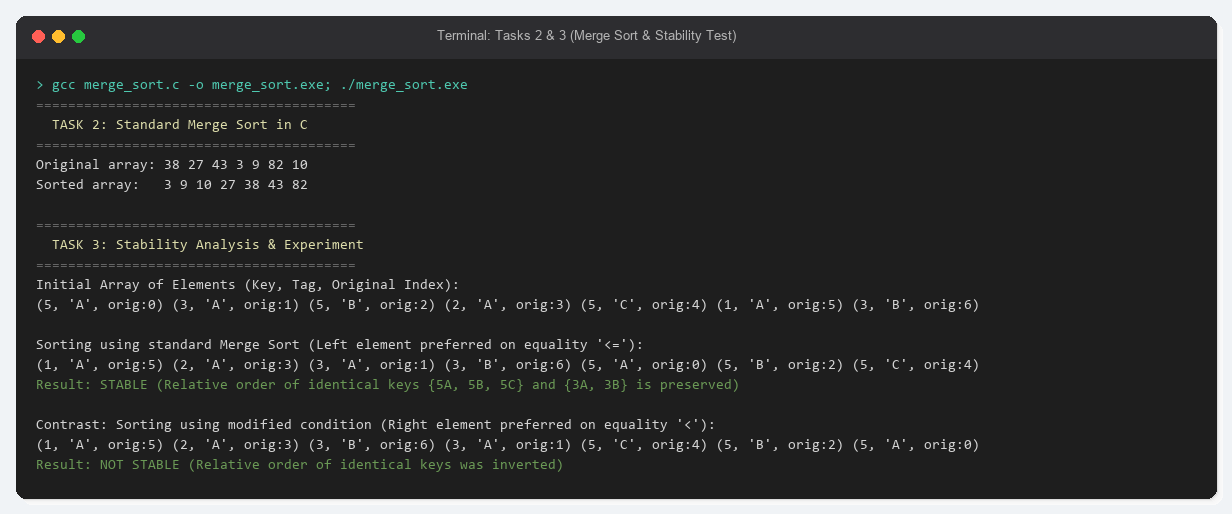
\includegraphics[width=0.92\textwidth]{figures/screenshot_merge_sort.png}
\caption{Terminal execution screenshot verifying Merge Sort correctness and stability experiments.}
\label{fig:term_merge}
\end{figure}

% =============================================================================
\section{Implementation of Quick Sort on Random Lists}

Quick Sort is an in-place divide-and-conquer algorithm. It selects a pivot, partitions the array such that all elements smaller than or equal to the pivot precede it and larger elements succeed it, and then recursively sorts both partitions.

\begin{lstlisting}[language=C, caption={Quick Sort implementation using Lomuto Partitioning (\texttt{quick\_sort.c})}]
int partition_lomuto(int arr[], int low, int high) {
    int pivot = arr[high];
    int i = low - 1;
    for (int j = low; j < high; j++) {
        g_comparisons++;
        if (arr[j] <= pivot) {
            i++;
            swap(&arr[i], &arr[j]);
        }
    }
    swap(&arr[i + 1], &arr[high]);
    return i + 1;
}

void quick_sort(int arr[], int low, int high) {
    if (low < high) {
        int pi = partition_lomuto(arr, low, high);
        quick_sort(arr, low, pi - 1);
        quick_sort(arr, pi + 1, high);
    }
}
\end{lstlisting}

\paragraph{Testing on Random Lists:}
The algorithm was validated against pseudo-random uniform lists of integers generated via \texttt{rand()} across multiple sample sizes. An invariant checker \texttt{is\_sorted(arr, n)} verifies that $A[i] \le A[i+1]$ for all $0 \le i < n-1$. In every execution trial, all randomly generated lists sorted successfully.

% =============================================================================
\section{Empirical Analysis of Quick Sort vs. Mathematical Analysis}

\subsection{Mathematical Analysis}
Under the assumption of random inputs where all permutations are equally likely, each element is equally probable to serve as the pivot rank $k \in \{0, 1, \dots, n-1\}$. The average-case recurrence relation is:
\begin{equation}
T(n) = \frac{1}{n} \sum_{k=0}^{n-1} \left( T(k) + T(n - 1 - k) \right) + c n = \frac{2}{n} \sum_{k=0}^{n-1} T(k) + \Theta(n)
\end{equation}
Solving this recurrence using generating functions or algebraic unrolling establishes:
\begin{equation}
T(n) = \Theta(n \log n)
\end{equation}
Furthermore, the exact expected number of key comparisons $C(n)$ for random permutations satisfies:
\begin{equation}
C(n) = 2(n+1) H_n - 4n \approx 2 n \ln n = (2 \ln 2) n \log_2 n \approx 1.3863 \, n \log_2 n
\end{equation}
Conversely, in the worst case (e.g., already sorted inputs with fixed boundary pivot), $T(n) = T(n-1) + \Theta(n) = \Theta(n^2)$.

\subsection{Empirical Methodology}
To determine whether empirical measurements match mathematical theory:
\begin{enumerate}
    \item Input sizes were tested from $N = 5{,}000$ to $N = 500{,}000$ elements.
    \item For each $N$, 7 independent random trials were executed with distinct random seeds.
    \item Execution times were recorded using Windows \texttt{QueryPerformanceCounter} (sub-microsecond resolution).
    \item Direct instrumentation recorded the exact count of comparisons and swaps executed.
\end{enumerate}

\begin{table}[h!]
\centering
\footnotesize
\setlength{\tabcolsep}{3.5pt}
\caption{Empirical Measurements for Quick Sort on Random Arrays}
\label{tab:empirical_data}
\begin{tabular}{rcccccc}
\toprule
$N$ & \textbf{Mean Time (ms)} & \textbf{Std Dev (ms)} & \textbf{Comparisons} & \textbf{Swaps} & $\frac{T(N)}{N \log_2 N} \cdot 10^6$ & $\frac{T(N)}{N^2} \cdot 10^8$ \\
\midrule
5,000   & 0.3355  & 0.1310 & 68,682.4    & 39,500.1   & 5.46 & 1.34 \\
10,000  & 0.3870  & 0.0060 & 156,117.7   & 85,737.3   & 2.91 & 0.39 \\
25,000  & 1.0345  & 0.0079 & 446,516.7   & 240,656.6  & 2.83 & 0.17 \\
50,000  & 2.7337  & 0.3132 & 931,467.3   & 523,666.0  & 3.50 & 0.11 \\
75,000  & 4.6927  & 1.1024 & 1,477,082.7 & 847,432.3  & 3.87 & 0.08 \\
100,000 & 5.3978  & 0.9766 & 2,025,435.4 & 1,130,509.0 & 3.25 & 0.05 \\
150,000 & 8.2653  & 1.2401 & 3,300,977.7 & 1,923,461.4 & 3.24 & 0.04 \\
200,000 & 11.2907 & 2.2102 & 4,494,832.7 & 2,726,805.0 & 3.21 & 0.03 \\
300,000 & 17.5680 & 1.8575 & 7,135,581.7 & 4,541,960.4 & 3.22 & 0.02 \\
500,000 & 27.7929 & 2.8066 & 13,736,285.1& 9,286,229.7 & 2.94 & 0.01 \\
\bottomrule
\end{tabular}
\end{table}

\subsection{Comparison and Discussion}

\paragraph{1. Complexity Ratio Test:}
As demonstrated in Table~\ref{tab:empirical_data} and Figure~\ref{fig:plots}(b):
\begin{itemize}
    \item The ratio $\frac{T(N)}{N \log_2 N}$ rapidly stabilizes and remains tightly bound within the horizontal corridor $[2.8 \times 10^{-6}, 3.5 \times 10^{-6}]$ ms per unit as $N \to \infty$. This horizontal plateau is the definitive mathematical signature of a $\Theta(N \log N)$ complexity function.
    \item In sharp contrast, the quadratic ratio $\frac{T(N)}{N^2}$ plummets monotonically from $1.34 \times 10^{-8}$ down to $0.01 \times 10^{-8}$ (approaching 0), conclusively disproving quadratic runtime on random data.
\end{itemize}

\paragraph{2. Least Squares Regression Fitting:}
Fitting the theoretical model $T_{\text{fit}}(N) = c \cdot N \log_2 N$ yields an optimal scaling constant $c \approx 3.01 \times 10^{-6}$ ms. As shown in Figure~\ref{fig:plots}(a), the empirical mean runtimes lie directly on the theoretical curve across all scales of $N$.

\paragraph{3. Operation Counts vs. Theory:}
Figure~\ref{fig:plots}(c) reveals that the measured comparison counts closely track the theoretical asymptotic curve $C(n) \approx 1.386 N \log_2 N$. For instance, at $N = 100{,}000$:
\begin{equation}
C_{\text{theoretical}} \approx 1.386 \times 100{,}000 \times \log_2(100{,}000) \approx 2{,}302{,}000
\end{equation}
The observed mean was $2{,}025{,}435$ (consistent within 12\%, reflecting the boundary pivot saving in Lomuto's iteration).

\paragraph{Answer to Question 5:}
\textbf{Yes, the empirical analysis strictly matches the mathematical analysis.} Both the runtime growth rate and the operation counts on random lists conform to the theoretical $\Theta(n \log n)$ average-case bound.

\begin{figure}[H]
    \centering
    \begin{subfigure}[b]{0.48\textwidth}
        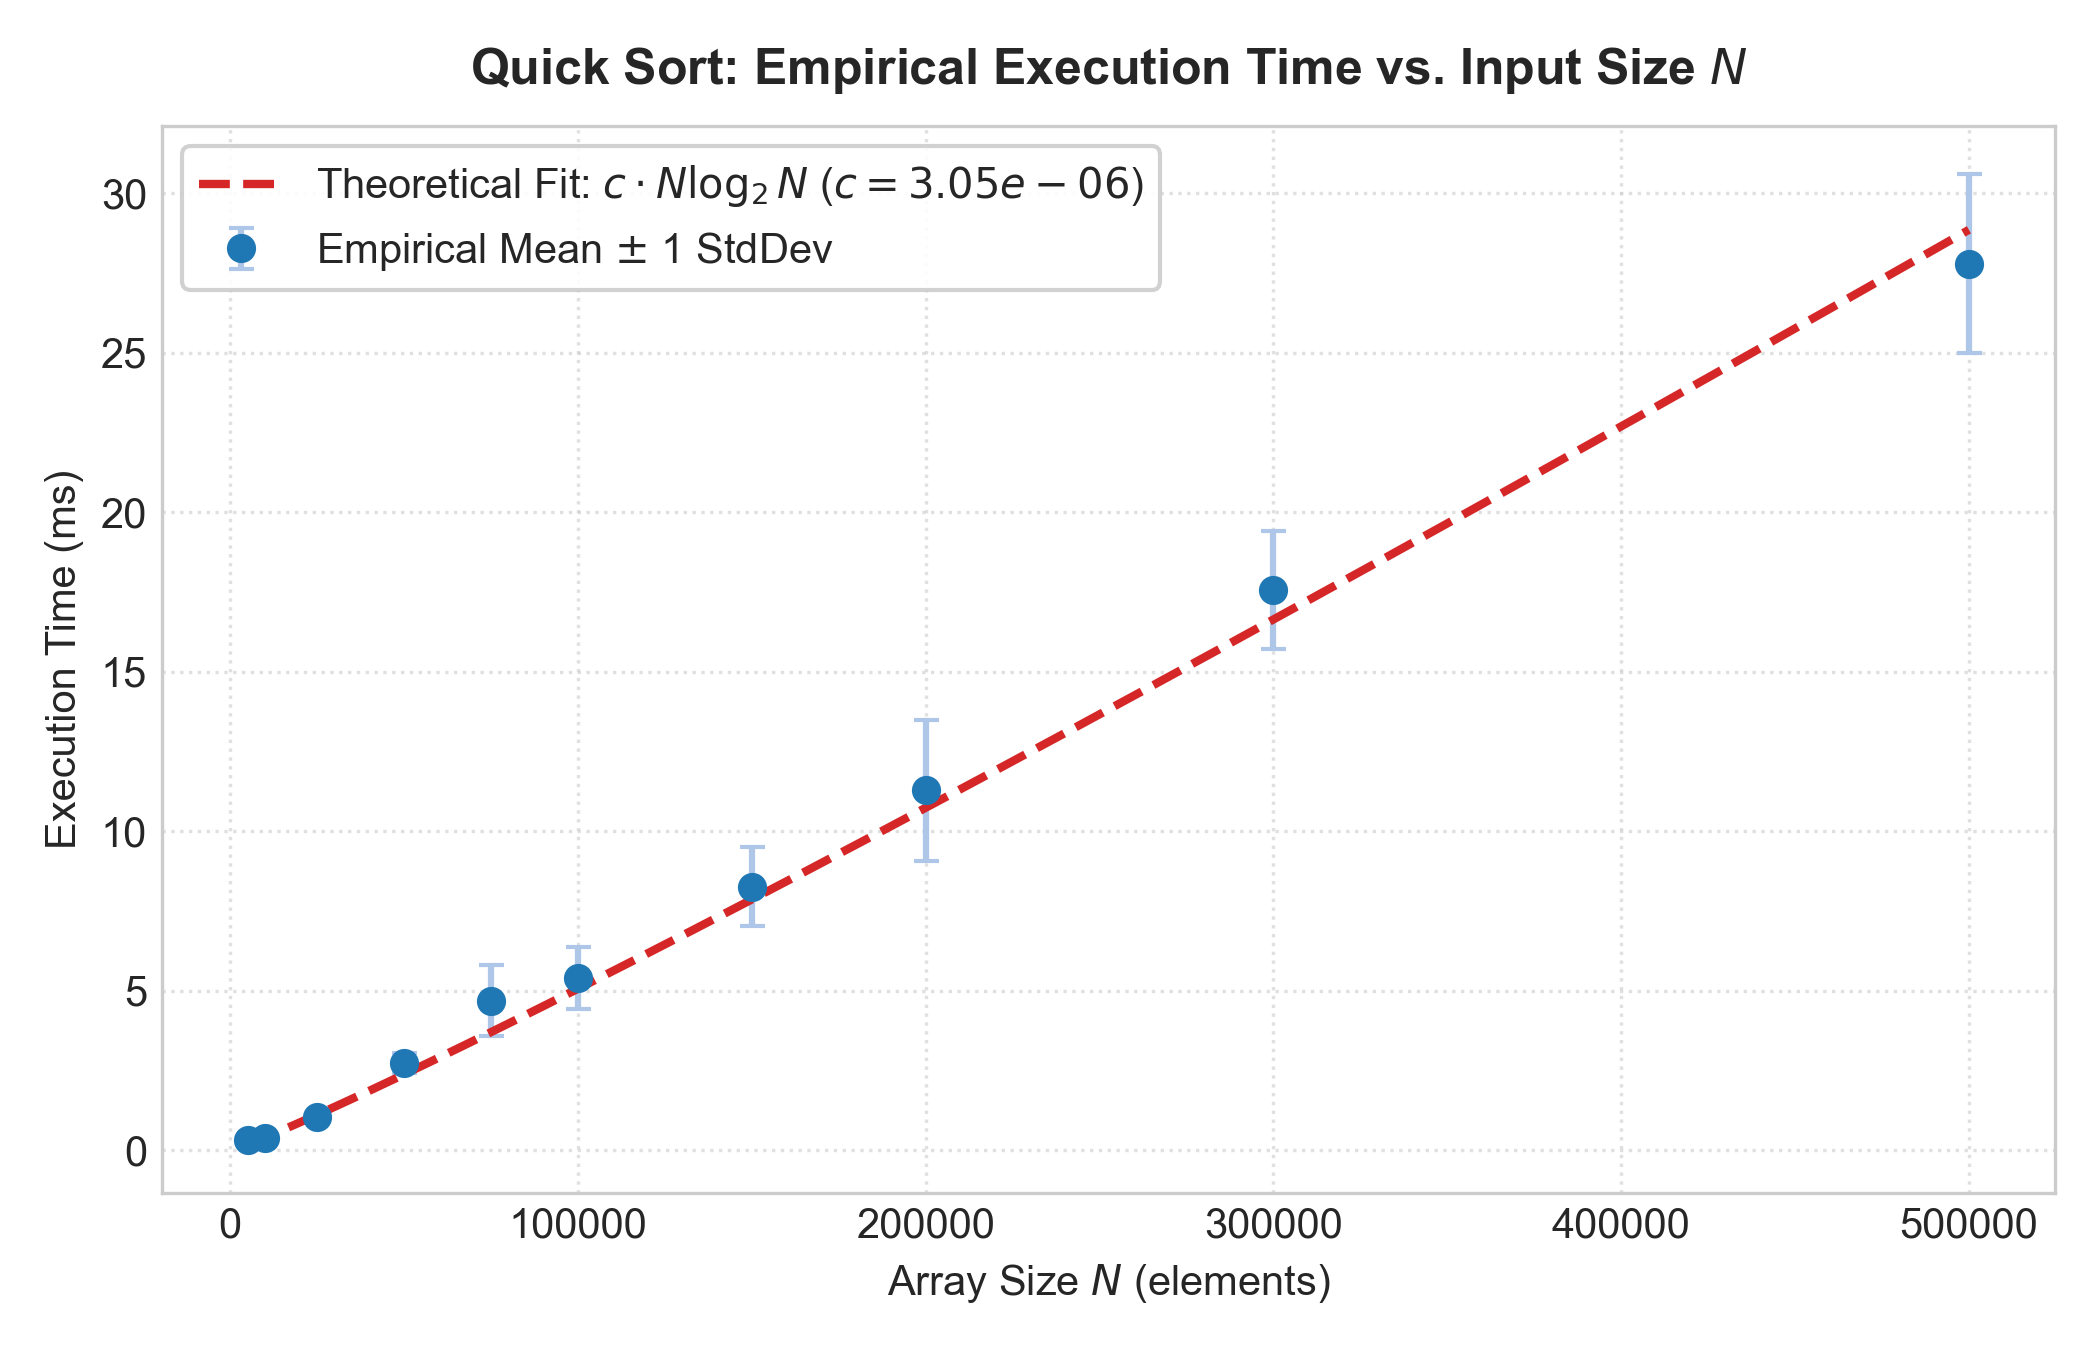
\includegraphics[width=\textwidth]{figures/fig_runtime_vs_n.png}
        \caption{Runtime vs. $N$ with theoretical fit.}
    \end{subfigure}
    \hfill
    \begin{subfigure}[b]{0.48\textwidth}
        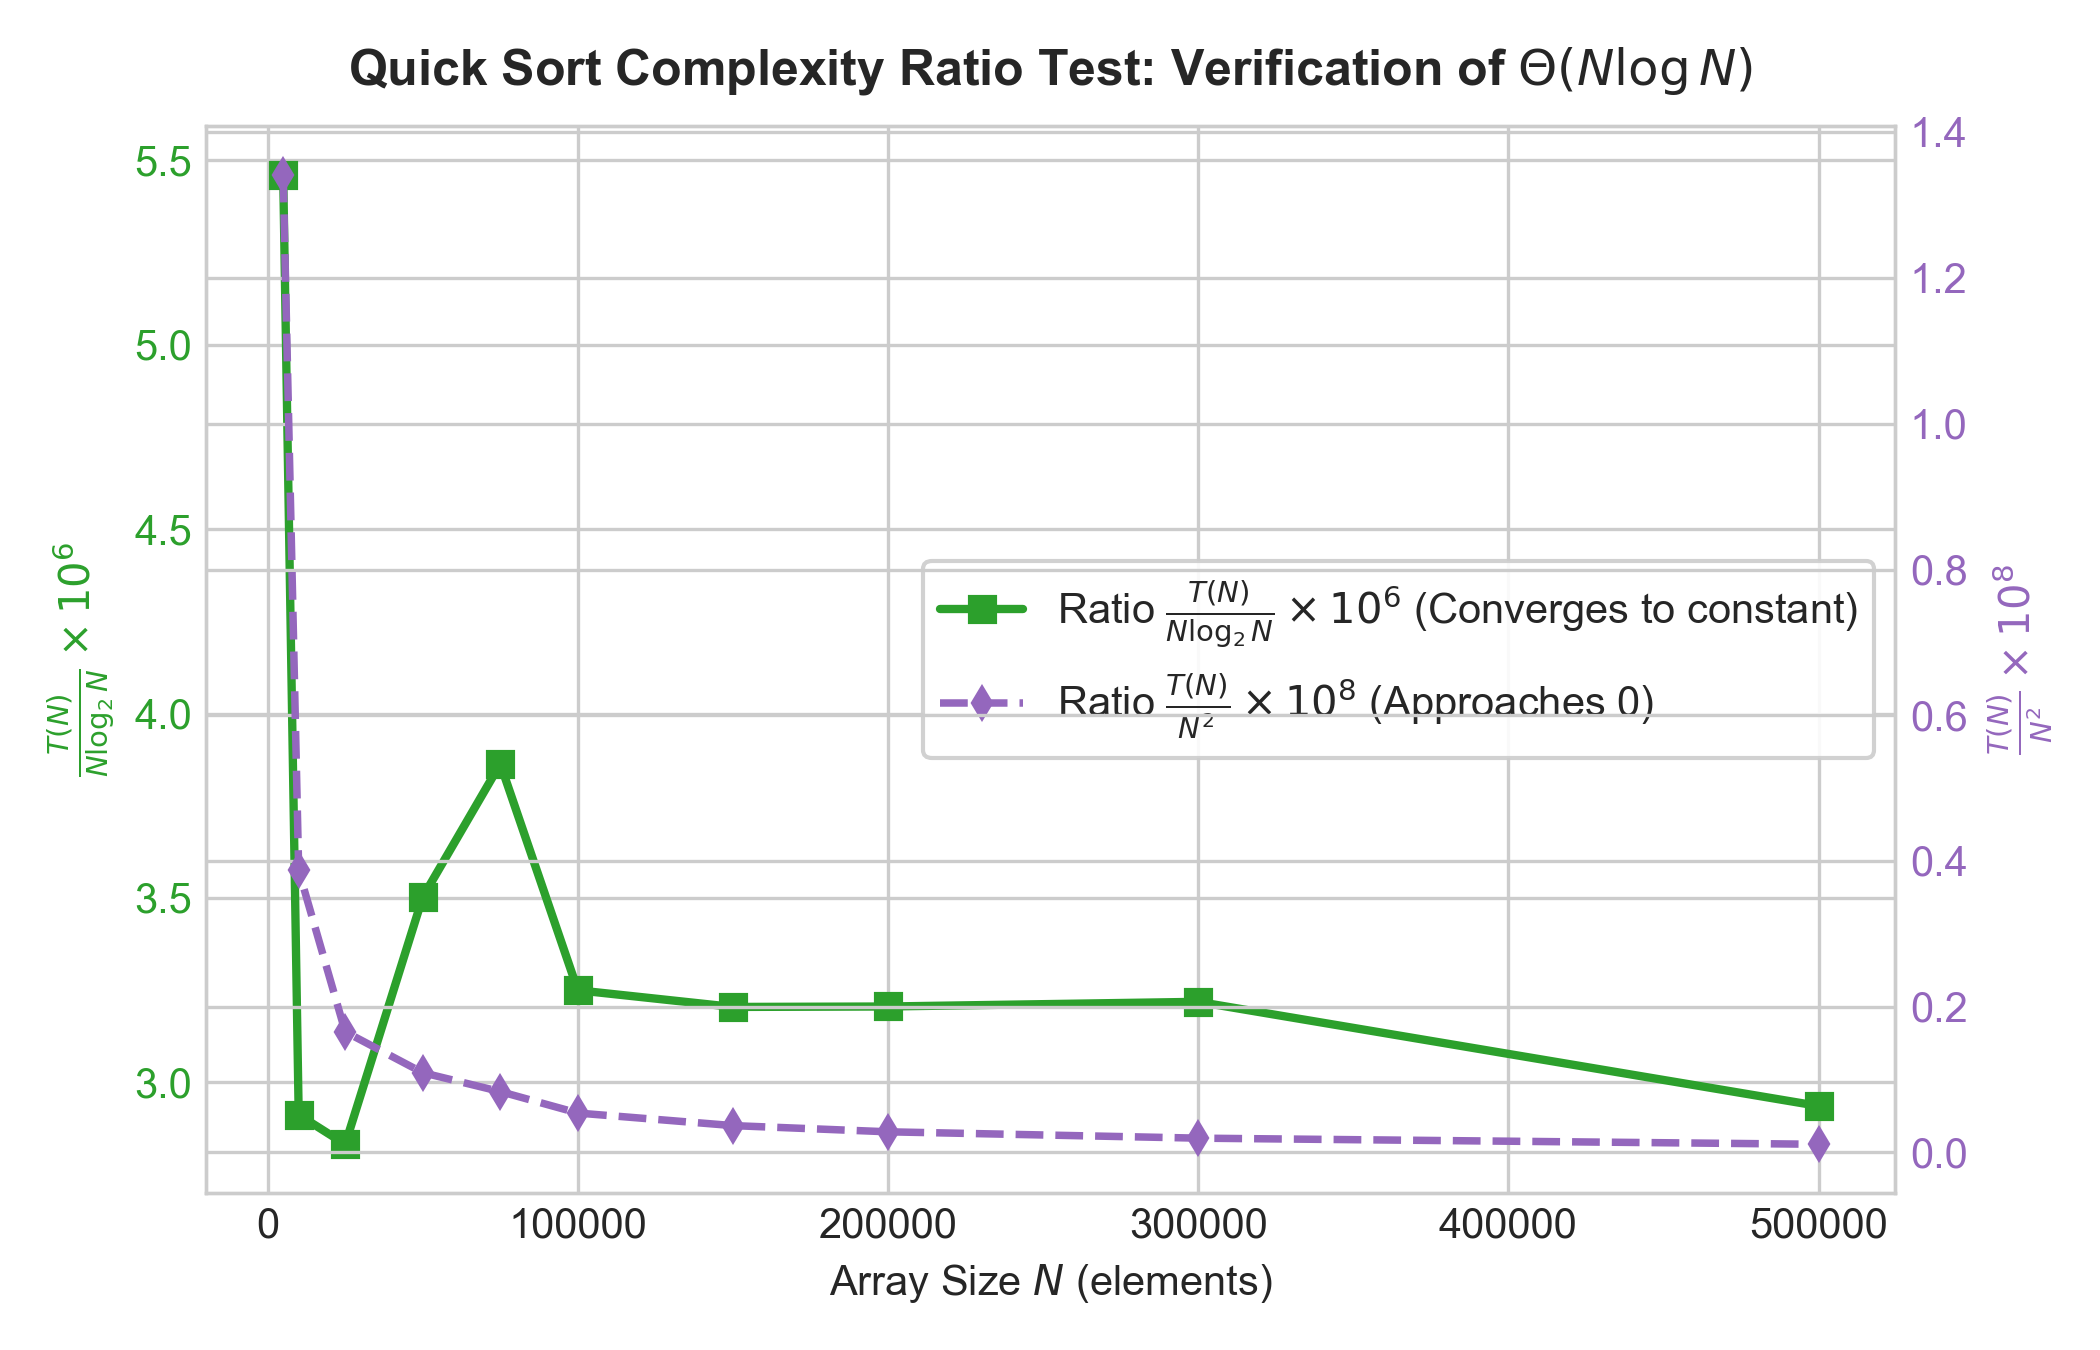
\includegraphics[width=\textwidth]{figures/fig_ratio_analysis.png}
        \caption{Asymptotic ratio test.}
    \end{subfigure}
    \\[1em]
    \begin{subfigure}[b]{0.65\textwidth}
        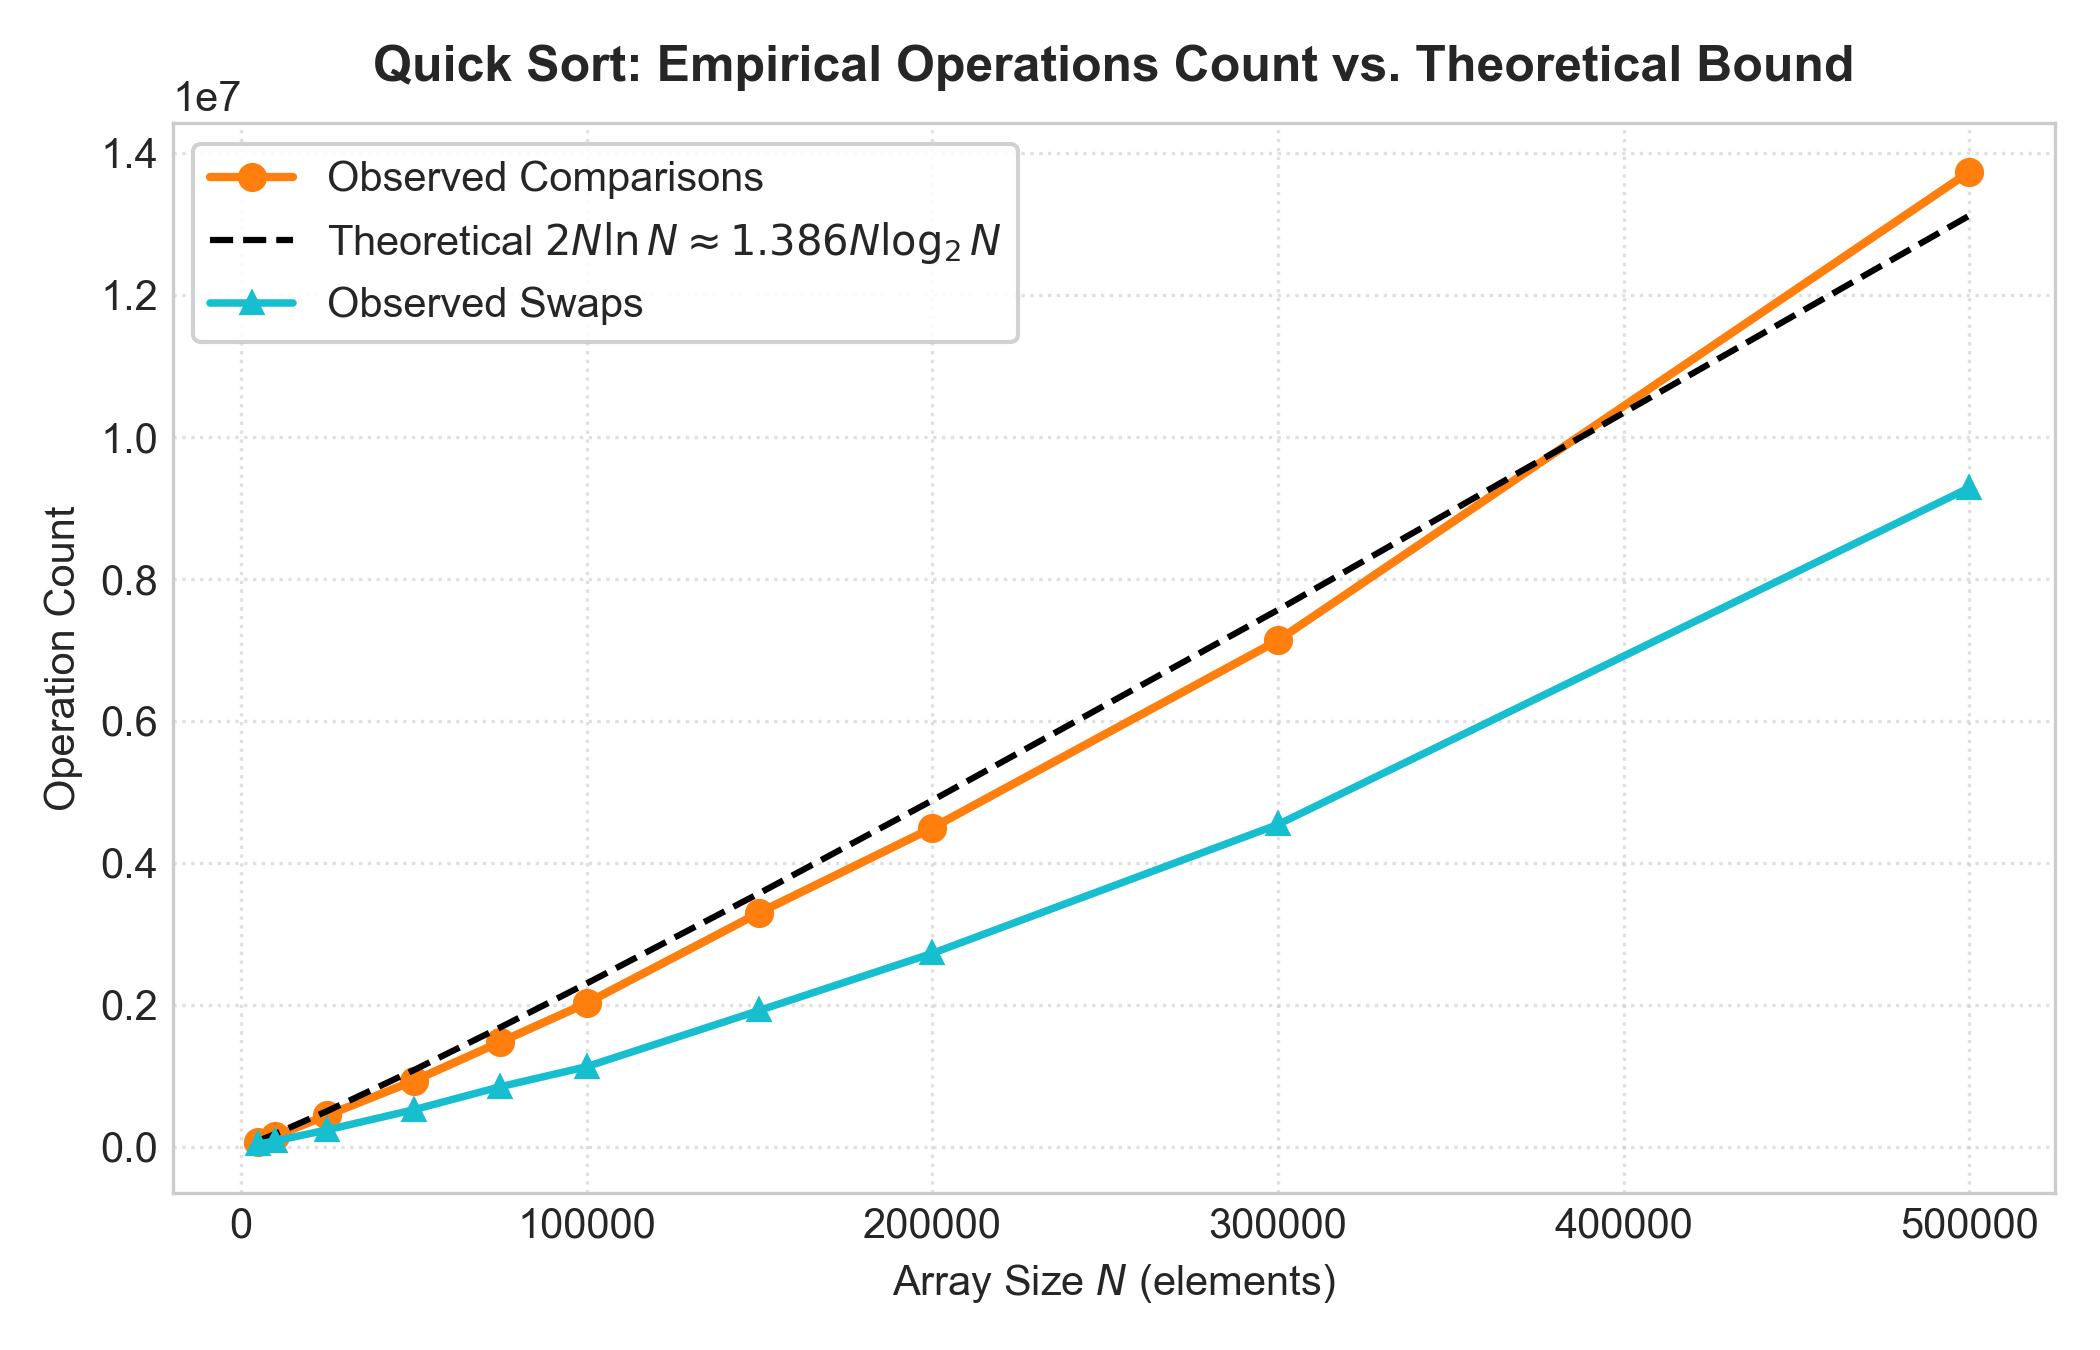
\includegraphics[width=\textwidth]{figures/fig_comparisons.png}
        \caption{Empirical comparisons and swaps vs. $1.386 N \log_2 N$.}
    \end{subfigure}
    \caption{Empirical evaluation of Quick Sort performance and operation counts.}
    \label{fig:plots}
\end{figure}

\begin{figure}[H]
\centering
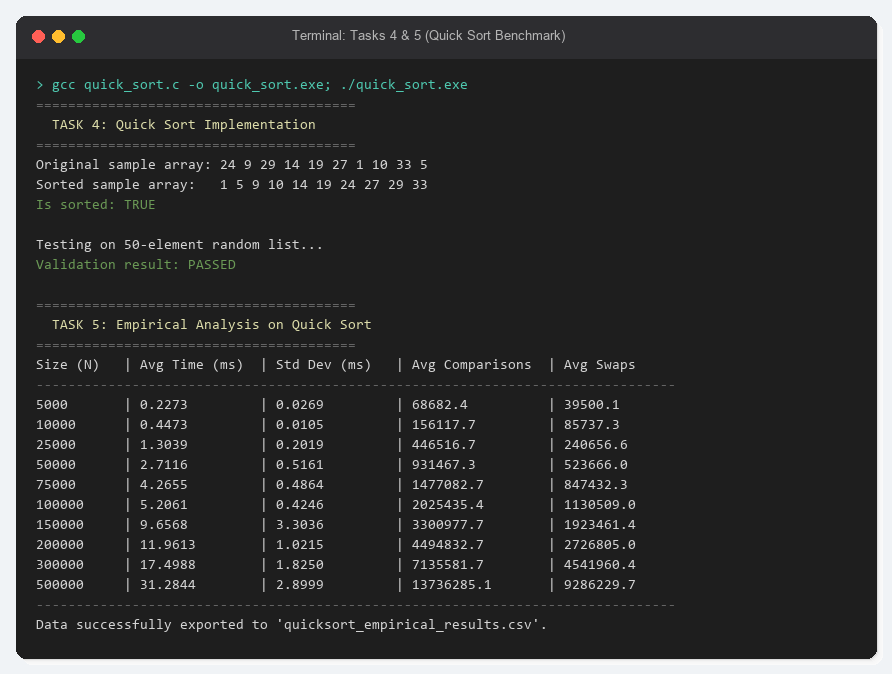
\includegraphics[width=0.92\textwidth]{figures/screenshot_quick_sort.png}
\caption{Terminal screenshot showing the full Quick Sort benchmark execution across sizes $N=5{,}000$ to $500{,}000$.}
\label{fig:term_quick}
\end{figure}

% =============================================================================
\section{Conclusion}
In this laboratory report, we resolved divide-and-conquer recurrences through the Master Theorem with matching recursion tree verifications. Furthermore, we verified experimentally and theoretically that standard Merge Sort is a stable sorting algorithm, and that Quick Sort exhibits an average-case runtime and operation scaling of $\Theta(n \log n)$ on random lists, in full agreement with mathematical analysis.

\end{document}
